\documentclass[10pt,a4paper]{article}
% Preamble of the thick-cylinder study report
\usepackage[T1]{fontenc}
\usepackage[utf8]{inputenc}
\usepackage{lmodern}
\usepackage[english]{babel}
\usepackage{microtype}
\usepackage[margin=22mm]{geometry}
\usepackage{amsmath,amssymb,mathtools}
\usepackage{bm}
\usepackage{booktabs}
\usepackage{array}
\usepackage{xcolor}
\usepackage{caption}
\usepackage{subcaption}
\usepackage{tikz}
\usepackage{pgfplots}
\pgfplotsset{compat=1.18}
\usepgfplotslibrary{groupplots}
\usepackage[numbers,sort&compress]{natbib}
\usepackage[colorlinks=true,linkcolor=blue!50!black,citecolor=green!40!black,
            urlcolor=blue!50!black]{hyperref}
\usepackage[nameinlink,capitalise]{cleveref}

\captionsetup{font=small,labelfont=bf}

% data folders (relative to report/)
\newcommand{\tab}{../results/tables}
\newcommand{\pdat}{../mesh/plotdata}

% notation
\newcommand{\PM}{\textsf{PM}}
\newcommand{\PP}{\textsf{PP}}
\newcommand{\PH}{\textsf{PH}}
\newcommand{\eE}{e_{\mathrm{E}}}
\newcommand{\eL}{e_{\mathrm{L}^2}}
\newcommand{\en}{e_{\mathrm{n}}}
\newcommand{\dd}{\,\mathrm{d}}
\newcommand{\bx}{\bm{x}}
\newcommand{\bxi}{\bm{\xi}}

% colours for p = 2..8 (sequential, dark = high p)
\definecolor{p2}{HTML}{FDB863}
\definecolor{p3}{HTML}{F08B3E}
\definecolor{p4}{HTML}{D9541A}
\definecolor{p5}{HTML}{B2182B}
\definecolor{p6}{HTML}{7F1C6A}
\definecolor{p7}{HTML}{4A2A8A}
\definecolor{p8}{HTML}{1B2A5E}

\pgfplotsset{
  conv/.style={
    xmode=log, ymode=log, x dir=reverse,
    width=4.6cm, height=4.6cm,
    xtick={1,0.5,0.25,0.125}, xticklabels={$1$,$\frac12$,$\frac14$,$\frac18$},
    xmin=0.1, xmax=1.25,
    ymin=1e-15, ymax=1e2,
    ytick={1e-14,1e-11,1e-8,1e-5,1e-2,1e1},
    tick label style={font=\scriptsize}, label style={font=\small},
    title style={font=\small, yshift=-1ex},
    unbounded coords=jump, mark size=1.3pt, line width=0.7pt,
    grid=major, grid style={gray!20},
  },
  pline/.style={color=p#1, mark=*, mark options={solid,fill=p#1}},
  pdash/.style={color=p#1, mark=o, dashed, mark options={solid}},
  phyb/.style={color=p#1, mark=square*, dashdotted, mark options={solid, fill=p#1}},
  meshplot/.style={
    width=3.35cm, height=3.35cm, axis equal image, hide axis,
    xmin=-0.05, xmax=3.05, ymin=-0.05, ymax=3.05,
    title style={font=\scriptsize, yshift=-1.2ex},
  },
}

% the same styles for TikZ paths (legends drawn outside the axes)
\tikzset{
  pline/.style={color=p#1, line width=0.7pt},
  pdash/.style={color=p#1, dashed, line width=0.7pt},
  phyb/.style={color=p#1, dashdotted, line width=0.7pt},
}

% h-convergence panel: #1 problem, #2 form, #3 alpha (3 digits), #4 key (eE, eL, eN)
\newcommand{\hpanel}[4]{%
  \foreach \pp in {2,...,8}{%
    \edef\tmp{\noexpand\addplot[pline=\pp] table[x=h, y=#4\pp] {\tab/h_#1_#2_a#3.dat};}\tmp
  }%
}
% slope triangle: #1 x-start (h), #2 y at x-start, #3 slope
\newcommand{\slope}[3]{%
  \draw[gray, thin] (axis cs:#1,#2) -- (axis cs:#1/2,#2/2^#3) -- (axis cs:#1,#2/2^#3) -- cycle;
  \node[gray, font=\tiny, anchor=west] at (axis cs:#1,{#2/2^(#3/2)}) {#3};
}

\usetikzlibrary{calc}
\renewcommand{\tab}{../results}

\title{Reproduction of the nodal rotation patch test and the convergence test of
       Rajendran (2010) for $\theta\ge90^\circ$ with the USEM code base}
\author{USEM-MATLAB study \texttt{studies/rajendran\_panel}}
\date{\today}

\begin{document}
\maketitle

\begin{abstract}
\noindent
The square-panel tests of \citet[Secs.~5.5--5.7]{Rajendran2010technique} (mid-side nodes
rotated by $\theta=90^\circ$--$270^\circ$, overlapping and folded elements) are recomputed
with the spectral elements of the code base on \texttt{Gmsh} meshes. With the 9-node element defined
as in the paper (parametric test functions, metric trial functions in Cartesian coordinates,
9th node at the centroid of the corners, $5\times5$ Gauss points), all values of the 9-node
Tables~15--19 are reproduced to four digits, for the unsymmetric (PM-QUAD9$^\ast$) as well as
the conventional (PP-QUAD9) and the metric (MM-QUAD9) elements, except for entries that are
inconsistent within the paper itself (\cref{sec:paper}). The energy-norm convergence rates of
PM-QUAD9$^\ast$ (Fig.~15 of the paper) are reproduced as well ($2.00$ and $1.98$ against
$2.11$ and $1.97$). For polynomial degrees $p\ge3$ the unsymmetric spectral element (\PM)
reproduces the cubic field of the shear test on every mesh, including fully folded ones, up to
round-off. The hybrid trial space of the code base (\PH: metric polynomials only for the
polynomials $P_p(\bx)$ of total degree $\le p$ in the Cartesian coordinates $\bx$, parametric
functions for the remainder) passes the constant and linear strain patch tests at $p=2$ on all meshes, converges
with rates $2.02$ and $2.21$ on sequences B and C, and reproduces the cubic field for $p\ge3$; at $p=8$
its round-off level on Meshes c and e is $220$--$260$ times lower than that of \PM. The code base
places all new nodes with the map of the 8-node (Serendipity) element, so the geometry stays
quadratic for every $p$ (subparametric elements for $p>2$); on these meshes this makes interior
and edge nodes coincide for even $p$. The code base now stops with an error in this case and when
the metric interpolation is singular, instead of returning a wrong (zero) solution
(\cref{sec:code}).
\end{abstract}

\section{Set-up}\label{sec:setup}
Panel $[0,2]\times[-1,1]$, plane stress, Poisson's ratio $\nu=0.25$, three point supports
(displacements $u_x=0$ at $(0,\pm1)$, $u_x=u_y=0$ at $(0,0)$), equilibrated loads on $x=0$ and
$x=2$, given by the normal stress $\sigma_x$ and the shear stress $\tau_{xy}$ (tension
$\sigma_x=1000$; moment $\sigma_x=-1500y$; shear $\sigma_x=-1500(2-x)y$,
$\tau_{xy}=750(1-y^2)$), displacement at $A=(2,0)$ (\cref{fig:setup}a--d). The meshes
(\cref{fig:meshes}) are generated with \texttt{Gmsh} (\texttt{mesh/gen\_panel\_meshes.py}):
$N\times N$ super-elements of $2\times2$ 8-node elements each. In every super-element, the
mid-side nodes of the four internal edges are rotated counter-clockwise about the centre node
of the super-element by the \emph{distortion angle} $\theta$, i.e., they move on the circle
through their original positions (\cref{fig:setup}e); $\theta=0^\circ$ is the undistorted
mesh, and the internal edges become parabolas through the rotated nodes. Meshes a--f consist of
a single super-element ($N=1$) with
$\theta=0^\circ,90^\circ,135^\circ,175^\circ,225^\circ,270^\circ$; the sequences A, B, C use
$\theta=0^\circ,90^\circ,135^\circ$ with $N=1,2,4$, i.e., $1\times1$, $2\times2$, $4\times4$
super-elements. For $\theta\ge90^\circ$ every element of every mesh has $\det(\bm J)\le0$
somewhere, where $\bm J$ is the Jacobian matrix of the element map.

\begin{figure}[t]
  \centering
  % Set-up of the panel tests of Rajendran (2010), Secs. 5.5-5.7 (adapted from
% manuscript/figures/fig-panel.tex): (a) panel [0,2] x [-1,1], supports
% u_x(0,+-1) = 0 and u(0,0) = 0 (rp_model.m), output point A = (2,0);
% (b)-(d) the three load cases, equilibrated tractions on x = 0 and x = 2
% (rp_loads.m, rp_exact.m), arrows to scale within each case (shear tractions
% in (d) with their own scale); (e) super-element of 2 x 2 8-node elements:
% the four internal mid-side nodes are rotated counter-clockwise by theta
% about the centre node (schematic, theta = 135 deg).
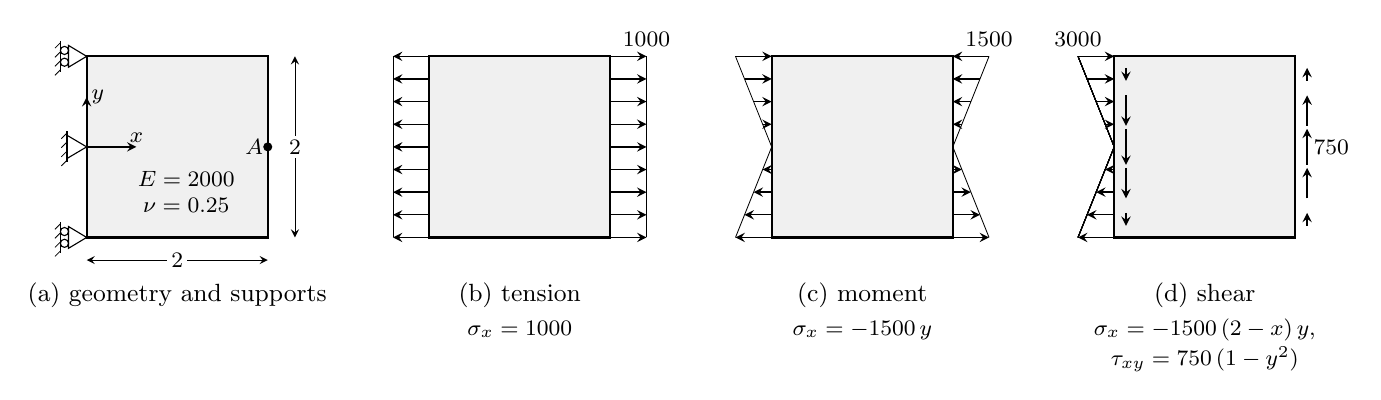
\begin{tikzpicture}[x=1.15cm, y=1.15cm,
    plabel/.style={anchor=north, font=\small, inner sep=0pt, align=center},
    slabel/.style={font=\footnotesize, inner sep=1.5pt},
    body/.style={draw=black, fill=gray!12, line width=0.8pt},
    trac/.style={-stealth, line width=0.5pt},
    roller/.pic={% apex at the node, restrains the displacement in the pic's x direction
      \draw[line width=0.4pt, fill=white] (0,0) -- (-0.2,0.12) -- (-0.2,-0.12) -- cycle;
      \draw[line width=0.4pt] (-0.245,0.065) circle (0.045) (-0.245,-0.065) circle (0.045);
      \draw[line width=0.6pt] (-0.29,0.17) -- (-0.29,-0.17);
      \foreach \s in {-0.15,-0.05,0.05,0.15} \draw[line width=0.3pt] (-0.29,\s) -- (-0.35,\s-0.06);},
    pin/.pic={% apex at the node, restrains both displacements
      \draw[line width=0.4pt, fill=white] (0,0) -- (-0.22,0.13) -- (-0.22,-0.13) -- cycle;
      \draw[line width=0.6pt] (-0.22,0.17) -- (-0.22,-0.17);
      \foreach \s in {-0.15,-0.05,0.05,0.15} \draw[line width=0.3pt] (-0.22,\s) -- (-0.28,\s-0.06);}]
% traction arrow at (#1,#2) on an edge with outward normal (#3,0), scaled
% traction (#4,#5): tail at the edge for tension, head at the edge for pressure
\def\panTrac#1#2#3#4#5{%
  \pgfmathsetmacro\pdn{(#4)*(#3)}%
  \pgfmathsetmacro\plen{veclen(#4,#5)}%
  \ifdim\plen pt>0.01pt
    \ifdim\pdn pt<0pt \draw[trac] ({#1-(#4)},{#2-(#5)}) -- (#1,#2);
    \else \draw[trac] (#1,#2) -- ++({#4},{#5});
    \fi
  \fi}
% (a) geometry and supports
\begin{scope}
  \draw[body] (0,-1) rectangle (2,1);
  \draw[-stealth, line width=0.5pt] (0,0) -- (0.55,0) node[slabel, above] {$x$};
  \draw[-stealth, line width=0.5pt] (0,0) -- (0,0.55) node[slabel, right] {$y$};
  \pic at (0,1) {roller};
  \pic at (0,-1) {roller};
  \pic at (0,0) {pin};
  \fill (2,0) circle (0.05) node[slabel, left] {$A$};
  \node[slabel, align=center] at (1.1,-0.5) {$E=2000$\\$\nu=0.25$};
  \draw[stealth-stealth, line width=0.3pt] (0,-1.25) -- node[slabel, fill=white] {$2$} (2,-1.25);
  \draw[stealth-stealth, line width=0.3pt] (2.3,-1) -- node[slabel, fill=white] {$2$} (2.3,1);
  \node[plabel] at (1,-1.5) {(a) geometry and supports};
\end{scope}
% (b) tension: sigma_x = 1000
\begin{scope}[xshift=4.35cm]
  \draw[body] (0,-1) rectangle (2,1);
  \foreach \y in {-1,-0.75,...,1} {
    \panTrac{2}{\y}{1}{0.4}{0}
    \panTrac{0}{\y}{-1}{-0.4}{0}}
  \draw[line width=0.3pt] (2.4,-1) -- (2.4,1) (-0.4,-1) -- (-0.4,1);
  \node[slabel, anchor=south, yshift=2pt] at (2.4,1) {$1000$};
  \node[plabel] at (1,-1.5) {(b) tension\\[1pt]\footnotesize $\sigma_x=1000$};
\end{scope}
% (c) pure bending: sigma_x = -1500 y (net moment 1000)
\begin{scope}[xshift=8.7cm]
  \draw[body] (0,-1) rectangle (2,1);
  \foreach \y in {-1,-0.75,...,1} {
    \panTrac{2}{\y}{1}{-0.4*\y}{0}
    \panTrac{0}{\y}{-1}{0.4*\y}{0}}
  \draw[line width=0.3pt] (2.4,-1) -- (2,0) -- (2.4,1) (-0.4,-1) -- (0,0) -- (-0.4,1);
  \node[slabel, anchor=south, yshift=2pt] at (2.4,1) {$1500$};
  \node[plabel] at (1,-1.5) {(c) moment\\[1pt]\footnotesize $\sigma_x=-1500\,y$};
\end{scope}
% (d) end shear: sigma_x = -1500 (2-x) y, tau_xy = 750 (1-y^2) (shear force 1000)
\begin{scope}[xshift=13.05cm]
  \draw[body] (0,-1) rectangle (2,1);
  % normal component on x = 0: t_x = 3000 y
  \foreach \y in {-1,-0.75,...,1}
    \panTrac{0}{\y}{-1}{0.4*\y}{0}
  \draw[line width=0.3pt] (-0.4,-1) -- (0,0) -- (-0.4,1);
  \node[slabel, anchor=south, yshift=2pt] at (-0.4,1) {$3000$};
  % shear component (own scale): t_y = 750 (1-y^2) on x = 2, -750 (1-y^2) on x = 0
  \foreach \y in {-0.8,-0.4,0,0.4,0.8} {
    \draw[trac] (2.13,{\y-0.2*(1-\y*\y)}) -- (2.13,{\y+0.2*(1-\y*\y)});
    \draw[trac] (0.13,{\y+0.2*(1-\y*\y)}) -- (0.13,{\y-0.2*(1-\y*\y)});}
  \node[slabel, right] at (2.15,0) {$750$};
  \node[plabel] at (1,-1.5) {(d) shear\\[1pt]\footnotesize $\sigma_x=-1500\,(2-x)\,y$,\\\footnotesize $\tau_{xy}=750\,(1-y^2)$};
\end{scope}
\end{tikzpicture}\par\bigskip
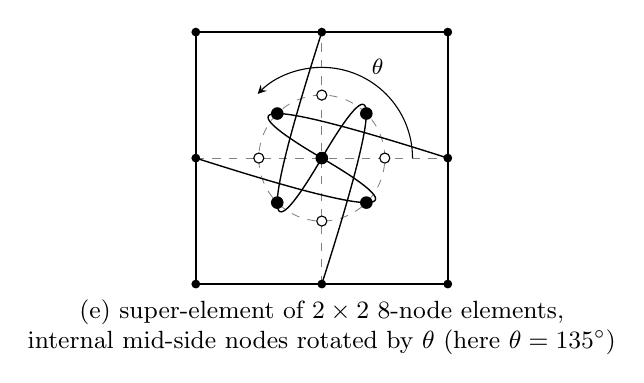
\begin{tikzpicture}[x=1.6cm, y=1.6cm,
    plabel/.style={anchor=north, font=\small, inner sep=0pt, align=center},
    slabel/.style={font=\footnotesize, inner sep=1.5pt}]
% (e) super-element of 2 x 2 elements: internal mid-side nodes rotated by theta
\def\th{135}
\draw[gray, dashed, line width=0.3pt] (-1,0) -- (1,0) (0,-1) -- (0,1);
\draw[gray, dashed, line width=0.3pt] (0,0) circle (0.5);
\foreach \k in {0,90,180,270}
  \draw[black, line width=0.5pt] plot[domain=-1:1, samples=41, variable=\s]
    ({0.5*cos(\k+\th)*(1-\s*\s) + cos(\k)*\s*(\s+1)/2},
     {0.5*sin(\k+\th)*(1-\s*\s) + sin(\k)*\s*(\s+1)/2});
\draw[line width=0.8pt] (-1,-1) rectangle (1,1);
\foreach \k in {0,90,180,270} {
  \draw[fill=white, line width=0.4pt] ({0.5*cos(\k)},{0.5*sin(\k)}) circle (0.04);
  \fill ({0.5*cos(\k+\th)},{0.5*sin(\k+\th)}) circle (0.05);
  \fill ({cos(\k)},{sin(\k)}) circle (0.035);}
\foreach \x/\y in {-1/-1,1/-1,1/1,-1/1} \fill (\x,\y) circle (0.035);
\fill (0,0) circle (0.05);
\draw[-stealth, line width=0.4pt] (0.72,0) arc[start angle=0, end angle=\th, radius=0.72];
\node[slabel, anchor=south west] at ({0.72*cos(60)},{0.72*sin(60)}) {$\theta$};
\node[plabel] at (0,-1.12) {(e) super-element of $2\times2$ 8-node elements,\\
  internal mid-side nodes rotated by $\theta$ (here $\theta=135^\circ$)};
\end{tikzpicture}

  \caption{Set-up of the panel tests \citep[Secs.~5.5--5.7]{Rajendran2010technique}:
    (a) geometry, supports and output point $A$; (b)--(d) load cases with the equilibrated
    tractions on $x=0$ and $x=2$ (arrows to scale within each case, the shear tractions in (d)
    with their own scale); (e) definition of the distortion angle $\theta$: the mid-side nodes
    of the internal edges (open circles at $\theta=0^\circ$) are rotated counter-clockwise by
    $\theta$ about the centre node of the super-element (filled dots).}
  \label{fig:setup}
\end{figure}

\paragraph{Material constant.} The paper states Young's modulus $E=1500$, but its exact solutions ($1.0$,
$1.5$, $3.3125$) are those of $E=2000$ (elasticity solutions with the supports above: $1.333$,
$2.0$, $4.4167$ for $E=1500$; $1.0$, $1.5$, $3.3125$ for $E=2000$). $E=2000$ is used here; all
displacements scale with $1/E$.

\paragraph{Loads.} The consistent nodal forces (\texttt{matlab/rp\_loads.m}) agree with the
lists of the paper (Fig.~8 and Sec.~5.6) except for the moment case of Fig.~8, where the
paper lists $-250$, $-500$ at nodes 8, 9 (and $250$, $500$ at nodes 14, 13); the consistent,
antisymmetric values are $-500$, $-250$ (and $500$, $250$). The listed values would give a
moment of $1125$ instead of $1000$; since the paper's PM9 results equal the exact $1.5$, the
consistent values were evidently used.

\paragraph{Elements.} With the polynomial degree $p=2$ (9 nodes):
PP9 = conventional element; MM9 = metric functions on both sides, element stiffness matrix
$\int\limits_{\hat\Omega}\bm B_{\mathrm R}^\top\bm D\bm B_{\mathrm R}\det(\bm J)\dd\xi\dd\eta$;
PM9 = PM-QUAD9$^\ast$, element stiffness matrix
$\int\limits_{\hat\Omega}(\bm B_{\mathrm L}^\ast)^\top\bm D\bm B_{\mathrm R}\dd\xi\dd\eta$. Here
$\hat\Omega=[-1,1]^2$ is the reference square with the coordinates $(\xi,\eta)$, $\bm D$ the
elasticity matrix, $\bm B_{\mathrm R}$ and $\bm B_{\mathrm L}$ the strain-displacement matrices of
the metric trial functions and the parametric test functions, and
$\bm B_{\mathrm L}^\ast=\bm B_{\mathrm L}\det(\bm J)$. As in the
paper: metric functions from $Q_2$ (polynomials of degree $\le2$ in each coordinate) in Cartesian
coordinates relative to the element centroid
(\texttt{ShapeFunctions2D\_Metric}, method 0), 9th node at the centroid of the corners,
$5\times5$ Gauss points. In addition: ``\PM, skew'' = the code-base metric functions (skew
coordinates, method 1) with the same nodes; ``\PM, code'' = \texttt{Ke\_2D} with the nodes of
\texttt{pSpectralElement\_NodesTopology} ($4\times4$ points). For $p=3,\dots,8$: \PP\ and \PM\
with interior nodes from the bilinear corner map (the generalisation of the corner centroid)
and $2p\times2p$ points, and \PM$_\mathrm{code}$ with the interior nodes of the code base. The
code-base metric functions are evaluated in the Lagrange basis on the bounding box of the skew
coordinates (default); the trial space is that of the monomial basis. \PH\ (hybrid trial space,
\texttt{ShapeFunctions2D\_Metric}, method 2): ``\PH, centr.'' with the 9th node at the corner
centroid and $5\times5$ points, ``\PH, code'' as ``\PM, code''; for $p\ge3$ \PH\ and
\PH$_\mathrm{code}$ analogous to \PM\ and \PM$_\mathrm{code}$.

\begin{figure}[t]
  \centering
  \begin{tikzpicture}
\begin{groupplot}[group style={group size=3 by 2, horizontal sep=0.05\textwidth, vertical sep=7mm}, scale only axis, width=0.3\textwidth, height=0.3\textwidth, hide axis, xmin=-0.03, xmax=2.03, ymin=-1.03, ymax=1.03, title style={font=\small, yshift=-0.5ex}]
\nextgroupplot[title={Mesh a: $\theta=0^\circ$}]
\addplot[black, line width=0.4pt] table {../mesh/plotdata/mesh_N1_t000.dat};
\nextgroupplot[title={Mesh b: $\theta=90^\circ$}]
\addplot[black, line width=0.4pt] table {../mesh/plotdata/mesh_N1_t090.dat};
\nextgroupplot[title={Mesh c: $\theta=135^\circ$}]
\addplot[black, line width=0.4pt] table {../mesh/plotdata/mesh_N1_t135.dat};
\nextgroupplot[title={Mesh d: $\theta=175^\circ$}]
\addplot[black, line width=0.4pt] table {../mesh/plotdata/mesh_N1_t175.dat};
\nextgroupplot[title={Mesh e: $\theta=225^\circ$}]
\addplot[black, line width=0.4pt] table {../mesh/plotdata/mesh_N1_t225.dat};
\nextgroupplot[title={Mesh f: $\theta=270^\circ$}]
\addplot[black, line width=0.4pt] table {../mesh/plotdata/mesh_N1_t270.dat};
\end{groupplot}
\end{tikzpicture}

\medskip

\begin{tikzpicture}
\begin{groupplot}[group style={group size=4 by 1, horizontal sep=0.04\textwidth, vertical sep=7mm}, scale only axis, width=0.22\textwidth, height=0.22\textwidth, hide axis, xmin=-0.03, xmax=2.03, ymin=-1.03, ymax=1.03, title style={font=\small, yshift=-0.5ex}]
\nextgroupplot[title={B, $2\times2$}]
\addplot[black, line width=0.4pt] table {../mesh/plotdata/mesh_N2_t090.dat};
\nextgroupplot[title={B, $4\times4$}]
\addplot[black, line width=0.4pt] table {../mesh/plotdata/mesh_N4_t090.dat};
\nextgroupplot[title={C, $2\times2$}]
\addplot[black, line width=0.4pt] table {../mesh/plotdata/mesh_N2_t135.dat};
\nextgroupplot[title={C, $4\times4$}]
\addplot[black, line width=0.4pt] table {../mesh/plotdata/mesh_N4_t135.dat};
\end{groupplot}
\end{tikzpicture}

  \caption{\texttt{Gmsh} meshes: Meshes a--f of the patch test (top) and the $2\times2$ and
    $4\times4$ meshes of sequences B ($\theta=90^\circ$) and C ($\theta=135^\circ$) (bottom),
    cf.\ Figs.~9, 10 of the paper.}
  \label{fig:meshes}
\end{figure}

\section{Nodal rotation patch test ($p=2$)}\label{sec:patch}
\begin{table}[h]
  \centering\small
  \caption{Moment loading, $u_y(A)$ (paper: Table~15; exact $1.5$).}
  \label{tab:moment}
  \resizebox{\linewidth}{!}{\begin{tabular}{l rr rr rr rr}
\toprule
 & \multicolumn{2}{c}{PP9} & \multicolumn{2}{c}{MM9} & \multicolumn{2}{c}{PM9 (PM-QUAD9$^\ast$)} & \multicolumn{2}{c}{\PM, $p=2$}\\
\cmidrule(lr){2-3}\cmidrule(lr){4-5}\cmidrule(lr){6-7}\cmidrule(lr){8-9}
mesh & present & paper & present & paper & present & paper & skew & code\\
\midrule
a (0$^\circ$) & 1.5000 & 1.5000 & 1.5000 & 1.5000 & 1.5000 & 1.5000 & 1.5000 & 1.5000\\
b (90$^\circ$) & 1.2606 & 1.2606 & 1.7935 & 1.7935 & 1.5000 & 1.5000 & 1.5000 & err.\\
c (135$^\circ$) & 1.0372 & 1.0372 & 1.6398 & 1.6398 & 1.5000 & 1.5000 & 1.5000 & 1.5000\\
d (175$^\circ$) & 1.2472 & 1.2472 & 1.5285 & 1.5285 & 1.5000 & 1.5000 & 1.5000 & 1.4996\\
e (225$^\circ$) & 1.0372 & 1.0372 & 1.6398 & 1.6398 & 1.5000 & 1.5000 & 1.5000 & 1.5000\\
f (270$^\circ$) & 1.2606 & 1.2606 & 1.7935 & 1.7935 & 1.5000 & 1.5000 & 1.5000 & err.\\
\bottomrule
\end{tabular}
}

  \vspace{3mm}
  \caption{Shear loading, $u_y(A)$ (paper: Table~16; exact $3.3125$). $^\ast$ after a paper value:
    differs from the present result, see \cref{sec:paper}.}
  \label{tab:shear}
  \resizebox{\linewidth}{!}{\begin{tabular}{l rr rr rr rr}
\toprule
 & \multicolumn{2}{c}{PP9} & \multicolumn{2}{c}{MM9} & \multicolumn{2}{c}{PM9 (PM-QUAD9$^\ast$)} & \multicolumn{2}{c}{\PM, $p=2$}\\
\cmidrule(lr){2-3}\cmidrule(lr){4-5}\cmidrule(lr){6-7}\cmidrule(lr){8-9}
mesh & present & paper & present & paper & present & paper & skew & code\\
\midrule
a (0$^\circ$) & 3.2979 & 3.2979 & 3.2979 & 3.2979 & 3.2979 & 3.2979 & 3.2979 & 3.2979\\
b (90$^\circ$) & 3.0033 & 1.9088$^\ast$ & 3.9559 & 3.9559 & 3.2710 & 3.2710 & 3.3120 & err.\\
c (135$^\circ$) & -0.4993 & -0.4993 & 3.8294 & 3.8294 & 3.3044 & 3.3044 & 3.4134 & 4.1224\\
d (175$^\circ$) & 2.5498 & 2.5498 & 3.3657 & 3.3657 & 3.3677 & 3.3677 & 3.1501 & 3.0340\\
e (225$^\circ$) & -0.4993 & -0.4993 & 3.8294 & 3.8294 & 3.3044 & 3.3044 & 3.4134 & 4.1224\\
f (270$^\circ$) & 3.0033 & 1.9088$^\ast$ & 3.9559 & 3.9559 & 3.2710 & 3.2710 & 3.3120 & err.\\
\bottomrule
\end{tabular}
}

  \vspace{3mm}
  \caption{Tension, $u_x(A)$ (paper: Table~14; exact $1.0$). $^\ast$ after a paper value: differs
    from the present result, see \cref{sec:paper}. In
    \cref{tab:moment,tab:shear,tab:tension,tab:conv}, ``err.'' marks cases in which the code base
    stops because interior and edge nodes coincide (\cref{sec:code}).}
  \label{tab:tension}
  \resizebox{\linewidth}{!}{\begin{tabular}{l rr rr rr rr rr}
\toprule
 & \multicolumn{2}{c}{PP9} & \multicolumn{2}{c}{MM9} & \multicolumn{2}{c}{PM9 (PM-QUAD9$^\ast$)} & \multicolumn{2}{c}{\PM, $p=2$} & \multicolumn{2}{c}{\PH, $p=2$}\\
\cmidrule(lr){2-3}\cmidrule(lr){4-5}\cmidrule(lr){6-7}\cmidrule(lr){8-9}\cmidrule(lr){10-11}
mesh & present & paper & present & paper & present & paper & skew & code & centr. & code\\
\midrule
a (0$^\circ$) & $1.0000$ & $1.0$ & $1.0000$ & $1.0$ & $1.0000$ & $1.0$ & $1.0000$ & $1.0000$ & $1.0000$ & $1.0000$\\
b (90$^\circ$) & $1.0000$ & $1.0$ & $1.1300$ & $1.0^\ast$ & $1.0000$ & $1.0$ & $1.0000$ & err. & $1.0000$ & err.\\
c (135$^\circ$) & $1.0000$ & $1.0$ & $1.4633$ & $1.0^\ast$ & $1.0000$ & $1.0$ & $1.0000$ & $1.0000$ & $1.0000$ & $1.0000$\\
d (175$^\circ$) & $1.0000$ & $1.0$ & $1.0285$ & $1.0^\ast$ & $1.0000$ & $1.0$ & $1.0000$ & $1.0000$ & $1.0000$ & $1.0000$\\
e (225$^\circ$) & $1.0000$ & $1.0$ & $1.4633$ & $1.0^\ast$ & $1.0000$ & $1.0$ & $1.0000$ & $1.0000$ & $1.0000$ & $1.0000$\\
f (270$^\circ$) & $1.0000$ & $1.0$ & $1.1300$ & $1.0^\ast$ & $1.0000$ & $1.0$ & $1.0000$ & err. & $1.0000$ & err.\\
\bottomrule
\end{tabular}
}
\end{table}
PM9 passes the constant and the linear strain patch tests on all meshes, as in the paper
(\cref{tab:tension,tab:moment}); for the quadratic-strain (cubic displacement) shear test, which
lies outside $Q_2$, its results are within $1.7\,\%$ of the exact value on all meshes
(\cref{tab:shear}). All PP9 and MM9 values for moment and shear coincide with the paper to four
digits, except for the entries marked $^\ast$. The metric functions of the code base (skew coordinates) give the same results for the
constant and linear strain tests and comparable ones for the shear test ($3.15$--$3.41$). \PH\
($p=2$, corner centroid) passes the constant and linear strain tests on all meshes as well, since
the polynomials $P_2(\bx)$ of total degree $\le2$ in the Cartesian coordinates $\bx$ are contained
in its trial space; for the shear test it is less accurate than PM9
($3.37$--$3.61$, i.e., $1.8$--$8.9\,\%$ error), because its quadratic complement is parametric.

\section{Convergence test (shear loading, $p=2$)}\label{sec:conv}
\begin{table}[h]
  \centering\small
  \caption{$u_y(A)$ for the sequences A, B, C (paper: Tables~17--19; exact $3.3125$). $^\ast$
    after a paper value: differs from the present result, see \cref{sec:paper}.}
  \label{tab:conv}
  \resizebox{\linewidth}{!}{\begin{tabular}{ll rr rr rr rr rr}
\toprule
 & & \multicolumn{2}{c}{PP9} & \multicolumn{2}{c}{MM9} & \multicolumn{2}{c}{PM9} & \multicolumn{2}{c}{\PM, $p=2$} & \multicolumn{2}{c}{\PH, $p=2$}\\
\cmidrule(lr){3-4}\cmidrule(lr){5-6}\cmidrule(lr){7-8}\cmidrule(lr){9-10}\cmidrule(lr){11-12}
seq. & mesh & present & paper & present & paper & present & paper & skew & code & centr. & code\\
\midrule
A & $1\times1$ & 3.2979 & 3.2979 & 3.2979 & 3.2979 & 3.2979 & 3.2979 & 3.2979 & 3.2979 & 3.2979 & 3.2979\\
 & $2\times2$ & 3.3106 & 3.3106 & 3.3106 & 3.3106 & 3.3106 & 3.3106 & 3.3106 & 3.3106 & 3.3106 & 3.3106\\
 & $4\times4$ & 3.3123 & 3.3123 & 3.3123 & 3.3123 & 3.3123 & 3.3123 & 3.3123 & 3.3123 & 3.3123 & 3.3123\\
\midrule
B & $1\times1$ & 3.0033 & 3.0033 & 3.9559 & 3.9559 & 3.2710 & 3.3044$^\ast$ & 3.3120 & err. & 3.3723 & err.\\
 & $2\times2$ & 3.1768 & 3.1768 & 3.9519 & 3.9519 & 3.3000 & 3.3057$^\ast$ & 3.3185 & err. & 3.3229 & err.\\
 & $4\times4$ & 3.2662 & 3.2661 & 3.9598 & 3.9598 & 3.3110 & 3.3116$^\ast$ & 3.3121 & err. & 3.3149 & err.\\
\midrule
C & $1\times1$ & -0.4993 & -0.4993 & 3.8294 & 3.8294 & 3.3044 & 3.2710$^\ast$ & 3.4134 & 4.1224 & 3.4016 & 3.0874\\
 & $2\times2$ & 2.9218 & 2.9218 & 3.9208 & 3.9208 & 3.3057 & 3.3001$^\ast$ & 3.2600 & 3.2935 & 3.3218 & 3.2938\\
 & $4\times4$ & 3.1531 & 3.1531 & 3.9660 & 3.9660 & 3.3116 & 3.3110$^\ast$ & 3.3067 & 3.3105 & 3.3121 & 3.3075\\
\bottomrule
\end{tabular}
}

  \vspace{3mm}
  \caption{Least-squares rates of the energy-norm strain error, Eq.~(24) of the paper (paper:
    Fig.~15). PP9 ($p=2$) and \PP\ ($p=3$) on folded meshes: the parametric strain is singular
    where $\det(\bm J)=0$, so the energy error of PP9 and \PP\ is not well defined for B and C
    (here: signed $\det(\bm J)$).
    ``--'': error at round-off level (field reproduced).}
  \label{tab:rates}
  \begin{tabular}{l rr rr rrrr}
\toprule
 & \multicolumn{2}{c}{PP9} & \multicolumn{2}{c}{PM9} & \PM, $p=2$ & \PM, $p=2$ & \PP, $p=3$ & \PM, $p=3$\\
\cmidrule(lr){2-3}\cmidrule(lr){4-5}
seq. & present & paper & present & paper & skew & code & & \\
\midrule
A & 1.99 & 1.93 & 1.99 & 1.93 & 1.99 & 1.99 & -- & --\\
B & 0.70 & 1.05 & 2.00 & 2.11 & 2.02 & 0.01 & 0.64 & --\\
C & 2.50 & 0.85 & 1.98 & 1.97 & 2.13 & 2.41 & 0.94 & --\\
\bottomrule
\end{tabular}

\end{table}
The displacements of sequence A and of PP9 and MM9 for B and C agree with the paper. PM9 on
sequence B yields the values the paper lists for sequence C and vice versa (\cref{sec:paper}).
PM9 converges with the optimal rate $2$ on the folded meshes of B and C (\cref{tab:rates}), as reported in the paper,
and so do \PM\ in skew coordinates ($2.02$, $2.13$) and \PH\ ($2.02$, $2.21$); PP9 does not ($0.70$,
$2.50$ from a negative displacement at $1\times1$). For $p=3$ both unsymmetric elements reproduce
the field on all meshes (error at round-off level, ``--''), whereas \PP\ ($p=3$) still has
energy-norm errors of $9$--$80\,\%$.

\section{Higher degrees}\label{sec:highp}
\begin{table}[h]
  \centering\small
  \caption{Shear loading on Meshes a--f: relative nodal error $\en$ for $p=3,\dots,8$ (cubic
    field, contained in the \PM\ trial space for $p\ge3$). \PM: interior nodes from the bilinear
    corner map; \PM$_\mathrm{code}$: interior nodes of \texttt{pSpectralElement\_NodesTopology};
    ``err.'': the code base stops (coincident nodes or singular metric interpolation).}
  \label{tab:highp}
  \begin{tabular}{lrrrrrr}
\toprule
 & a (0$^\circ$) & b (90$^\circ$) & c (135$^\circ$) & d (175$^\circ$) & e (225$^\circ$) & f (270$^\circ$)\\
\midrule
\PP, $p=3$ & 1e-14 & 2e-1 & 1e-1 & 2e-1 & 1e-1 & 2e-1\\
\PM, $p=3$ & 2e-14 & 2e-14 & 7e-14 & 1e-13 & 2e-14 & 3e-14\\
\PM$_\mathrm{code}$, $p=3$ & 7e-14 & 7e-13 & 1e-12 & 7e-8 & 6e-12 & 1e-13\\
\PH, $p=3$ & 3e-14 & 3e-14 & 3e-13 & 2e-13 & 2e-13 & 6e-13\\
\PH$_\mathrm{code}$, $p=3$ & 2e-14 & 5e-14 & 9e-14 & 6e-8 & 8e-14 & 1e-14\\
\addlinespace[2pt]
\PP, $p=4$ & 1e-13 & 8e-2 & 5e-1 & 2e-1 & 5e-1 & 8e-2\\
\PM, $p=4$ & 1e-13 & 2e-13 & 3e-12 & 3e-11 & 3e-12 & 2e-13\\
\PM$_\mathrm{code}$, $p=4$ & 1e-13 & err. & 3e-11 & err. & 5e-10 & err.\\
\PH, $p=4$ & 1e-13 & 2e-14 & 6e-12 & 5e-13 & 1e-11 & 1e-14\\
\PH$_\mathrm{code}$, $p=4$ & 1e-13 & err. & 1e-12 & err. & 1e-12 & err.\\
\addlinespace[2pt]
\PP, $p=5$ & 8e-13 & 7e-2 & 9e-2 & 2e-1 & 9e-2 & 7e-2\\
\PM, $p=5$ & 9e-13 & 1e-10 & 6e-13 & 8e-11 & 6e-13 & 3e-11\\
\PM$_\mathrm{code}$, $p=5$ & 8e-13 & 4e-10 & 8e-10 & err. & 6e-10 & 5e-9\\
\PH, $p=5$ & 9e-13 & 8e-13 & 2e-12 & 2e-11 & 5e-12 & 2e-13\\
\PH$_\mathrm{code}$, $p=5$ & 6e-13 & 7e-13 & 2e-12 & err. & 2e-12 & 2e-13\\
\addlinespace[2pt]
\PP, $p=6$ & 7e-13 & 9e-2 & 2e-1 & 1e-1 & 2e-1 & 9e-2\\
\PM, $p=6$ & 6e-13 & 1e-11 & 6e-11 & 3e-11 & 2e-11 & 1e-11\\
\PM$_\mathrm{code}$, $p=6$ & 6e-13 & err. & 1e-8 & err. & 7e-9 & err.\\
\PH, $p=6$ & 5e-13 & 2e-13 & 2e-11 & 1e-10 & 1e-11 & 2e-13\\
\PH$_\mathrm{code}$, $p=6$ & 4e-13 & err. & 2e-12 & err. & 2e-12 & err.\\
\addlinespace[2pt]
\PP, $p=7$ & 3e-13 & 1e-1 & 9e-2 & 1e-1 & 9e-2 & 1e-1\\
\PM, $p=7$ & 4e-14 & 2e-11 & 4e-10 & 8e-10 & 1e-9 & 4e-11\\
\PM$_\mathrm{code}$, $p=7$ & 3e-13 & 2e-6 & 8e-8 & err. & 4e-7 & 2e-6\\
\PH, $p=7$ & 5e-13 & 5e-12 & 1e-10 & 3e-10 & 2e-11 & 9e-12\\
\PH$_\mathrm{code}$, $p=7$ & 1e-12 & 2e-12 & 4e-12 & err. & 3e-11 & 2e-12\\
\addlinespace[2pt]
\PP, $p=8$ & 3e-12 & 1e-1 & 1e0 & 1e-1 & 1e0 & 1e-1\\
\PM, $p=8$ & 3e-12 & 3e-9 & 8e-6 & 1e-7 & 1e-5 & 5e-9\\
\PM$_\mathrm{code}$, $p=8$ & 3e-12 & err. & err. & err. & err. & err.\\
\PH, $p=8$ & 3e-12 & 1e-10 & 7e-8 & 6e-9 & 1e-8 & 4e-11\\
\PH$_\mathrm{code}$, $p=8$ & 2e-12 & err. & 1e-11 & err. & 3e-11 & err.\\
\bottomrule
\end{tabular}

\end{table}
With interior nodes from the bilinear corner map, both unsymmetric elements are
distortion-immune for $p=3,\dots,8$ (\cref{tab:highp}): the cubic field is reproduced on
all meshes with overlapping and folded elements. The round-off level grows with $p$ and
distortion, for \PM\ from $10^{-13}$ to $10^{-5}$ ($p=8$, Meshes c and e), for \PH\ to $8\cdot10^{-8}$,
in line with the thick-cylinder study. With the interior nodes of the code base, \PH\ is
computable in more cases than \PM\ (e.g., $p=8$, Meshes c and e: \PM$_\mathrm{code}$ rejected,
\PH$_\mathrm{code}$ $\en\le2\cdot10^{-11}$). The conventional element has errors of $7$--$100\,\%$ on
the distorted meshes for all $p$.

\section{Node placement of the code base}\label{sec:code}
\texttt{pSpectralElement\_NodesTopology} places all new nodes with the geometry map of the
original element, i.e., at the images of the Gauss-Lobatto-Legendre points under the bilinear map of a 4-node or
the quadratic map of an 8-node (Serendipity) element. The degree-$p$ element therefore keeps the
geometry of the input mesh for every $p$: the elements are subparametric for $p>2$, and the
higher-order terms of an isoparametric geometry description are never used. Increasing $p$ thus
improves the approximation of the displacements, but not that of the geometry. This is a
limitation of the code base, not a property of the method. Where the input mesh only
approximates a curved boundary, the geometry error stays that of the 8-node mesh under
$p$-refinement, and the nodes have to be placed on the exact geometry to obtain isoparametric
elements; the thick-cylinder study does this for the circular arcs outside the code base
(Gordon-Hall blending of the exact edges). On the panel meshes considered here, the boundary is
straight and the curved internal edges are part of the definition of the test, so the
geometry is represented exactly and the results of \cref{sec:patch,sec:conv,sec:highp} are not
affected by this limitation.

A second consequence concerns strongly distorted elements. On Meshes b and f, the 8-node map sends
the interior reference point $\bxi=(0,0)$ onto a mid-side node of the same element (e.g., in the
element with the corners $\bx_1=(0,-1)$, $\bx_2=(1,-1)$, $\bx_3=(1,0)$, $\bx_4=(0,0)$:
$-\tfrac14\sum\limits^{4}_{i=1}\bx_i+\tfrac12\sum\limits^{8}_{i=5}\bx_i=(1,-0.5)$, with the mid-side
nodes $\bx_5,\dots,\bx_8$), for every even $p$. No set of distinct nodes represents this element
geometry; the 9th node of the paper (corner centroid) defines a different geometry. Before commit
\texttt{da84a58} the metric Vandermonde matrix $\bm V$ was then singular
(condition number $\kappa(\bm V)\approx10^{18}$--$10^{20}$) and the computed displacements were silently zero.
Since then the code base keeps this node placement but stops with an error:
\texttt{pSpectralElement\_NodesTopology} on coincident nodes, and \texttt{ShapeFunctions2D\_Metric}
when its interpolation matrix is singular to working precision (reciprocal condition number
$\mathrm{rcond}$ below the machine epsilon, $\mathrm{rcond}<\varepsilon_{\mathrm{mach}}$),
which also covers the nearly non-unisolvent node sets of Meshes c--e for high $p$, where the
accuracy had been destroyed (\cref{tab:highp}). The ``code'' columns and
\PM$_\mathrm{code}$, \PH$_\mathrm{code}$ rows show these cases as ``err.''. With the Lagrange basis
of the metric functions (bounding box of the skew coordinates) the interpolation matrix is better
conditioned than with monomials: five \PM$_\mathrm{code}$ cases that the check rejected with the
monomial basis ($p=3$, Mesh d; $p=6,7$, Meshes c and e) are now computed and pass the patch test
($\en\le5\cdot10^{-7}$), and the round-off-dominated values change towards the exact ones (e.g.,
$p=2$, Mesh d, moment: $u_y(A)=1.49957\to1.50000$). On all meshes of the test suite, the
Lee \& Bathe input files and the thick-cylinder meshes with distortion angle $\alpha\le30^\circ$ ($p\le8$) neither
check is triggered. The study results with interior nodes from the bilinear corner map
(\PM, $p\ge3$) show that such meshes can be computed if a different geometry is acceptable.

\section{Inconsistencies in the paper}\label{sec:paper}
\begin{enumerate}
\item $E=1500$ is stated; the exact values correspond to $E=2000$ (\cref{sec:setup}).
\item Fig.~8, moment loading: nodal forces at nodes 8/9 and 14/13 interchanged (\cref{sec:setup}).
\item Table~16, PP-QUAD9, Meshes b and f: $1.9088$; the present value $3.0033$ equals the paper's
  own PP-QUAD9 value for the same mesh in Table~18 ($1\times1$ super-element of sequence B).
\item Tables~18 and 19, PM-QUAD9$^\ast$ columns: interchanged. The present values for sequence B
  ($3.2710$, $3.3000$, $3.3110$) are the paper's Table~19 entries ($3.2710$, $3.3001$, $3.3110$),
  those for C the Table~18 entries; the $1\times1$ values of Table~16 (b: $3.2710$, c: $3.3044$)
  confirm the present assignment.
\item Table~14, MM-QUAD9: $1.0$ for all meshes. With a stiffness matrix that reproduces all MM9
  moment and shear values to four digits, MM9 gives $1.1300$ (b, f), $1.4633$ (c, e), $1.0285$ (d),
  also with load vectors computed from the metric functions (Eq.~(22) of the paper). MM9 does not
  pass the constant strain patch test on these meshes; the paper's entries could not be reproduced.
\end{enumerate}
Apart from these items, every 9-node value of the paper for $\theta\ge90^\circ$ is reproduced to
four digits. The 8-node results (Tables~8--13) are not reproduced: the code base provides only
tensor-product (Lagrange) elements.

\section{Reproduction}
\texttt{mesh/gen\_panel\_meshes.py} (\texttt{Gmsh}), \texttt{matlab/rp\_run.m} (all computations,
\texttt{MATLAB} R2026a; code base of commit \texttt{af3e04f}), \texttt{postprocess.py} (tables and
mesh figure). Paper values: \texttt{results/paper\_values.csv}, \texttt{results/paper\_rates.csv}.

\bibliographystyle{plainnat}
\bibliography{../../../literature/references}
\end{document}
